%\documentclass[11pt]{amsart}
\documentclass[11pt]{article}
\usepackage{geometry}                % See geometry.pdf to learn the layout options. There are lots.
\geometry{letterpaper}                   % ... or a4paper or a5paper or ... 
%\geometry{landscape}                % Activate for for rotated page geometry
%\usepackage[parfill]{parskip}    % Activate to begin paragraphs with an empty line rather than an indent
\usepackage{graphicx}
\usepackage{subfigure}
\usepackage{amssymb}
\usepackage{epstopdf}
\usepackage{hyperref}
\usepackage{comment}
\DeclareGraphicsRule{.tif}{png}{.png}{`convert #1 `dirname #1`/`basename #1 .tif`.png}

\newcommand{\nuc}[2]{\ensuremath{^{#1}}#2}


\title{SLIMER Long Writeup\\
Version 1.0: \emph{Evidence For Observation of \nuc{14}{C}}
} 
\author{Steve Elliott,
Christopher Fowler,
Mary Kidd,
Michael Ronquest,
Erik Shaw
}


\begin{document}




\maketitle
\section{Introduction}
Permafrost underlies about 22-24\% of the Earth's surface.  Global climate models project the strongest future warming in the Northern Hemisphere high latitudes.  Thus, thawing permafrost and the resulting microbial decomposition of previously frozen organic carbon (C) is one of the most significant potential feedbacks from terrestrial ecosystems to the atmosphere.   There have been predictions that the decomposition of permafrost organic C will produce a significant feedback to global warming on a century timescale.  These estimates are based upon experiments performed at 30$^\circ$ C, not performed on permafrost materials and based upon homogenized samples, not intact active-layer/permafrost.  CH$_4$ has 25 times more greenhouse warming potential than CO$_2$ on a century timescale.  Increases in factors leading to deglaciation were followed by a rise in atmospheric CH$_4$ originating from  permafrost.  The concentration of atmospheric CH$_4$ appears to have risen over the last two years after a decade of stability. This increase may be related to unusually warm summers in Siberia, which harbors the largest reservoirs of permafrost C. 

Part of this study relies upon understanding the rate at which individuals in the microbial community in the permafrost samples ingest the organic carbon.The community will be divided by type onto a RNA/DNA microarray.  Each microbial type will be fluorescently tagged.The microbes will be fed a carbon substrate doped with $^{14}$C, which decays via beta decay.Our apparatus will detect the fluorescent light from the tags as well as the electrons emitted from the beta decay.  This has never been done in a single step process.

To summarize, our goal is to develop an apparatus that will read RNA/DNA microarrays and observe both the fluorescent tags from the samples and the electrons emitted from the $^{14}$C beta decay.  Each sample of RNA is distributed among wells that are 100$\times$100$\times$20 $\mu$m$^3$.  The samples are imaged with a cooled EMCCD camera and a wide-band fluorescence microscope.  We propose altering a microscope configuration to include sensitivity to electrons from the beta decay .  



\section{Description of the Apparatus}
\subsection{Microscope Body}
The body of the microscope is a Ti-U Eclipse Inverted Research Microscope from Nikon Instruments.  The inverted microscope indicates that the light source and condenser are above the sample pointing down, and the objectives and turret are below the sample pointing up.  (See Figure \ref{fig:light_path} for the light path)
\begin{figure}[h!p]
\centering
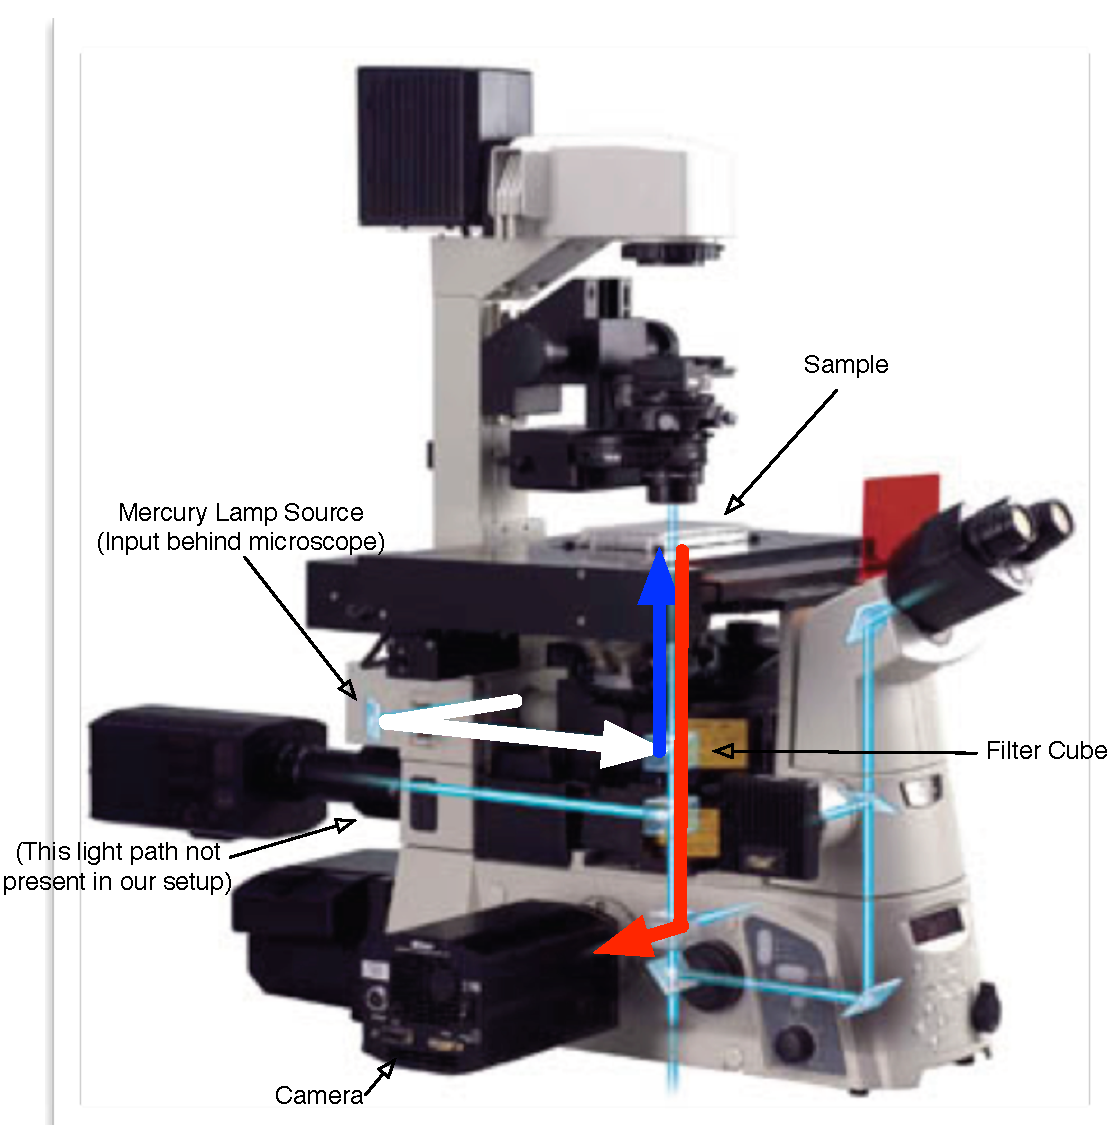
\includegraphics[width=\textwidth]{misc_plots/microscope-light-path.pdf}
\caption[Light Path]{(Color online.)  A cartoon of the light path through the microscope.)}
\label{fig:lightpath}
\end{figure}


\subsubsection{Fluorescence System}
The fluorescent light source, called the Intensillight, is a mercury (Hg) lamp which emits white light.  This light is transmitted to the microscope body via a delicate fiber optics cable.  Because the cable is easily damaged, a separate feedthrough was constructed for it in the dark box.  This feedthrough was designed to minimize any stress on the cable, so it is very close to the cable input to the Epi-fl illuminator.  

The lamp shutter can be controlled through the NIS Elements software or manually through a remote control.  The neutral density (ND) filters can also be inserted using the software or control.  These filters can cut the intensity of the light.  There is also a manual shutter located on the filter turret.

\subsubsection{Filter Cubes}
The fluorescent light travels from the Epi-fl illuminator to the filter turret where it encounters a filter cube.  The filter cube is designed to filter the incoming white light to the excitation frequency required and direct it upward toward the sample using a dichromatic beamsplitter.  The light emitted from the sample returns downward to the filter cube, but the emission filter (also called barrier filter) allows the emission frequency to pass through to the camera while blocking any reflected excitation light.  

The filters we purchased are very high-quality, high-transmission Semrock filters, which, as can be seen in Figure \ref{fig:filter}, transmit at $>$ 97\%.  If this filter cube is in place for $^{14}$C data collection, the transmission of the excitation light as well as the transmission of the dichroic mirror (about 96\%).  

%%%%%%%%%%%%%%%%%%%%
\begin{figure}
\centering
\includegraphics
%[width=3.5in]{setup-mod}
[width=5in]{filter_cube/semrock-fitc-3540C-NTE.pdf}
\caption[Filter Emission]{(Color online.)  This plot shows the transmission of the excitation and emission light in the Semrock FITC filter.  )}
\label{fig:filter}
\end{figure}
%%%%%%%%%%%%%%%%%%%%


\subsubsection{Lenses}
The objective lenses are Nikon's CFI Plan Fluor series.  These have an extra-high transmission rate ($>$85\%) and excellent flatness of field.  They are specifically designed for fluorescence observation and imaging.  We have magnifications of 4X, 10X, 20X, and 40X.  Each objective has  a different numerical aperture (NA), which is an indication of how much light is collected by the lens.  These are listed in Table \ref{tab:lens}.  From the numerical aperture, the resolving powers of these objectives can be calculated using $R = \frac{0.61\lambda}{NA}$ where $\lambda$ is the wavelength of light.  Here, the resolving power is calculated for $\lambda$=550 nm, the emission from CsI(Tl) (see Section \ref{sec:CsI}).  

The field of view (FOV) can be calculated by considering the 512$\times$512 effective area of the CCD.  Each pixel is 16 $\mu$m in width.  From there, it is a simple scaling argument to get the FOV for each objective:  $FOV = \frac{512\times16 \mu m}{X}$ where $X$ is the magnification factor.  This gives the width of the FOV in $\mu$m.  Finally, the FOV translates to a number of images required to cover the entire sample chip, which is 1.28 cm $\times$ 1.28 cm (see Section \ref{sec:phyla}).  This is a vital consideration since we will have to count for a specific length of time at each location, so the number of images required should be as low as possible.  

\begin{table}[t]\caption[]{Some useful values calculated for our four objectives.}
\begin{tabular}{|c|c|c|c|c|}
\hline
Objective & Numerical Aperture & R ($\mu$m) & Field of View (mm)  & Number of Images\\
\hline
 4X & 0.13 & 2.58  &  2.05  & 36\\\hline
 10X & 0.30 & 1.12  &  0.819 &  256 \\\hline
 20X & 0.50  & 0.67  &   0.410 & 961\\\hline
 40X & 0.75  & 0.45  & 0.205 & 3969\\\hline
 \end{tabular}
 \label{tab:lens}
\end{table}
\subsubsection{EMCCD Camera}
The camera used with this setup is an electron-multiplying charge-coupled device (EMCCD) by Photometrics.  The model is the Evolve$^-$.  The difference between the EMCCD and a traditional CCD lies in the use of an extended serial register.  Within this register, the signal electrons are accelerated from pixel to pixel via the application of a higher-than-normal CCD clock voltage.  Secondary electrons are then generated in the silicon by impact ionization, resulting in a magnification of the original signal.  The number of secondary electrons generated can be controlled by increasing or decreasing the clock voltage.  The camera can be operated in either traditional CCD mode (with no gain applied) or EM mode.  The camera is also equipped with three different readout speeds, 10 MHz, 5 MHz, and 1.25 MHz (the latter is only available in traditional CCD mode).   

\subsection{Scintillator}\label{sec:CsI}
CsI(Tl) is a very commonly used scintillation detector.  It has a high light output of about 40 photons/keV.  In $^{14}$C beta decay, the endpoint energy of the electron energy spectrum is 156.475 keV, and the mean energy of the emitted electrons is 49.47 keV.  Thus, a light yield of about 2000 photons can be expected for a typical electron.  We approximate that roughly 50\% of these exit the screen, though this is an underestimate.

The density of normal CsI is 4.51 g/cm$^3$, but due to the well-separated columnar structure, the density of columnar CsI(Tl) is reduced to 80\% of the full density.  Using the available online tools from the National Institute of Standards and Technology (NIST), the rate of electrons in CsI can be tabulated.  For a 50.00 keV electron, the range in g/cm$^2$ is 8.633$\times10^{-3}$, and for a 150.0 keV electron, the range is 5.206$\times10^{-2}$ g/cm$^2$.  Thus, a 50.00 keV electron will travel 23.9 $\mu$m, and a 150.0 keV electron will travel 144 $\mu$m.  

A thinner scintillator layer results in better spatial resolution.  If a thickness was chosen to stop roughly 80\% of the electrons emitted, the range corresponding to an 80.00 keV electron would be used, which corresponds to 52 $\mu$m. 

The transmission spectrum for CsI(Tl) is broad and includes many common excitation and emission frequencies, so that the fluorescence should not be drastically affected.  The emission spectrum is peaked around 550 nm, so the choice of fluorescent dye must take this into consideration.  




\subsection{Copper Collimators}
Two copper collimators were fabricated in order to assist with this study. 
One has diameter of 1 mm the other a diameter of 250 $\mu$m.
Their purpose is twofold: their ``shadow'' produces a region on the scintillator where no events should occur, and thus assist in cross-checks of the \nuc{14}{C} signal. Secondly, they provide a landmark which can be used to focus and align the microscope. Once the alignment and focus procedure are complete, the collimator aligns the calibration source to ensure that the FOV is within the central area of the source where the activity resides. 



\subsection{Source, Scintillator, Collimator (SSC) assembly}
In order to be more consistent with data taking, a holder for the source, scintillator and collimator was fabricated out of plastic. 
This holder permits reproducible alignment of the three, and prevents the collimator from moving when a source is placed.
It also prevents the collimator from bending the scintillator out of the focal plane of the microscope.   




\section{Recommended Procedure For Data Taking} % needs work
\subsection{Power-up procedure}
The equipment should be powered up in the following order:
\begin{enumerate}
\item Dia Illumination: switch is located on the external control box, however there is an extra set of controls on the microscope body.
\item Motorized Stage: switch is located on the external power supply box.
\item Fluorescence Light (if used): switch is located on the external light source. 
\item EMCCD: switch is on the camera body
\item Microscope Power: switch is on the microscope body, in the back and to the left near round accessory plug jacks.
\item Nikon Elements DAQ software: Select Roper Scientific driver. At this point, the operating temperature of the camera should be selected. 
\end{enumerate}
Once Elements has started, the camera will begin to cool. This make take some time, so the camera's temperature should be monitored in the camera dialog. Starting and stopping
image acquisition (live view is sufficient) will prompt the camera to be polled and its temperature updated. -80C is the lowest \emph{set} temperature that can be achieved, although setting the temperature to -90C  
will get down roughly to -85C. 

The filter wheel position should be checked, as this can impact light collection. To do this, Go to Devices $\rightarrow$ Manage Devices $\rightarrow$ Nikon Microscope. The list of installed equipment should include the filter turret. Select a consistent empty filter slot. 


\subsection{Recommended EMCCD and microscope settings}
For consistency, it is essential that the same settings be used for each run. The recommendations are:
\begin{description}
\item[Magnification] 20x, to improve light collection 
\item[EM Gain] 200, recommendation from Chris Murphy at Photometrics 
\item[BERT] Off, as this can be applied at the software level
\item[Electron Conversion Gain] 1/6x , seems to produce good results.
\item[Quant-View] Off
\item[Set Temperature] -90C, although it should be noted that the temperate never gets this low. Lower temperatures appear to produce a cleaner signal. 
\item[Actual Temperature] -84C or lower. 
\item[Readout Speed] 5MHz, the lowest possible when running with EM Gain, in order to decrease readout noise
%\item[Clear Cycles] 2 
\item[Exposure Time] 200ms, seems to produce good results
\item[Trigger] Internal Trigger 
\item[Keep Overlapped?] Selected
\item[Clear Mode] Grayed out by ``Keep Overlapped'' selection.
\item[Sensor Mode] Grayed out by ``Keep Overlapped" selection.
%\item[Clear Mode] Pre-exposure
%\item[Sensor Mode]  Frame Transfer 
\item[Filter Cube] For scintillation only counting, no filter cube should be used. 
\item[Dia Illumination] Confirmed as switched off, as it can produce low levels of light when on.
\end{description} 
% I deselected "Keep overlapped", and used "pre-exposure" clear modes.  Selecting "Frame Transfer" and "Pre-exposure" clearing will run the camera in non-overlapped mode. 





\subsection{Focusing Procedure}
When using a calibration source with the scintillator/collimator holder, the following focusing procedure is used:
\begin{enumerate}
\item Place the scintillator/collimator holder into the clamp located on the stage. The collimator should be in place. 
\item Rotate the correct objective into place. 
\item Begin live acquisition in NI Elements. 
\item Power up the Dia Illuminator, starting with low illumination and slowly increasing until light is seen in the live image. 
\item Adjust the fine and course focus knobs on the side of the microscope until dark ``dots'' can be seen, and appear to be in sharp focus. 
\item Once this is done, further adjust the illumination until the image is reasonably bright. 
\item Further adjust the fine focus until the hexagonal features on the CsI slide can be seen. 
\end{enumerate}
Once the bottom of the CsI slide is in focus, the calibration source may be placed in the collimator. 
\subsection{Data Taking Settings}
Data is taken in Time Lapse Acquisition Mode. Using a macro, data is collected in hour increments, then the output data file name is incremented. Doing so mitigates the 
amount of data lost in the event of a camera communication issue, as well as permits the resulting data files to be converted into a standard \verb+.tiff+ format using the Bio Formats library. 

\subsection{Fluorescence Measurements}
\emph{Procedure to be added.}


\subsection{Camera Calibration}
The camera's RapidCal feature is exploited for calibration purposes. The procedure is to open the dark box, and rotate the metallic silver collar around the camera's input port until the LED light comes on.
The LED will flash and change color until the RapidCal procedure is complete: at which point the LED will be solid green. This procedure may take some time if starting from a warm state (it must cool down first).
It should also be noted that the RapidCal will only activate if the camera is NOT in communication with the Nikon Elements software. 
The mapping of the LED state is as follows:
\begin{itemize}
\item Blinking Orange: cooling
\item Blinking Green: calibrating
\item Solid Green: calibration complete. 
\end{itemize}
RapidCal should be done once a week.


\section{Data Analysis} % needs work
The analysis code is written in Python, and utilizes a number of external libraries to enable reasonably fast analysis of data. These libraries include NumPy, SciPy, PANDAS as well as PIL. 
These may all be obtained within the Anaconda Python package \url{https://store.continuum.io/}. 

The DAQ software writes data into Nikon's proprietary data format \verb+nd2+. While the DAQ software can also export the data frame by frame into standard TIFF format, we have identified an open source package called Bio-Formats \url{http://loci.wisc.edu/software/bio-formats}, part of the Open Microscopy Environment \url{http://www.openmicroscopy.org/site} that can do the same. As Bio-Formats is written in java, it can be run on WIT, and is thus convenient.  
One drawback of Bio-Formats is that the conversion program, \verb+bfconvert+, loads the entire nd2 file into memory at once. It also invokes java with a memory limit of 512 MB. The bfconvert command has been modified to use up to 20GB of memory, with the modified command being \verb+bfconvert_very_large+. However, this tool is limited to converting files of 20GB in size or less.  

\subsection{Locations on WIT}
The copy of Anaconda, which includes the python distribution and libraries used in this analysis, can be setup on the Weak Interactions Team cluster WIT by sourcing this file:
\begin{verbatim}
                /proj/Software/Notes/SetupScripts/setup_anaconda_root.sh
\end{verbatim}
Note that this will also setup a copy of ROOT which can interact with the newer version of python. 

The Bio-Formats conversion tool is located here:
\begin{verbatim}
               /proj/Software/ImageProcessing/bftools/bfconvert
\end{verbatim}
while the modified version, able to operate on files up to 20GB in size, is located here:
\begin{verbatim}
               /proj/Software/ImageProcessing/bftools/bfconvert_very_large
\end{verbatim}

The simulation, done in RAT, can be found here:
\begin{verbatim}
               /proj/Slimer/SlimerSims/MySims/SimpleGeo
\end{verbatim}

The analysis codes can be found here:
\begin{verbatim}
                /home/ronquest/Work/SLIMER
\end{verbatim}
and is kept within a \verb+git+ repository. This repository can be checked out by doing this:
\begin{verbatim}
               git clone /home/ronquest/Work/SLIMER master
\end{verbatim}


\subsection{Analysis Chain}
The data flow, from data taking to final histograms is:
\begin{itemize}
	\item Nikon Elements Data Acquisition $\rightarrow$ a single \verb+.nd2+ file per run
	%\item  1 \verb+.nd2+ file per run $\rightarrow$ Nikon Elements Export to TIFF $\rightarrow$ N \verb+.tiff+ files, 1 per exposure 
	\item A single \verb+.nd2+ file per run $\rightarrow$ \verb+bfconvert+ $\rightarrow$ N \verb+.tiff+ files, 1 per exposure
	\item  Background \verb+.tiff+ files $\rightarrow$ \verb+background_average.py+ $\rightarrow$ a single \verb+.npz+ (NumPy Zip archive) file, which contains 2 \verb+ndarray+s representing the mean and variance for each pixel in the EMCCD camera
	\item Background  \verb+.npz+ file + data \verb+.tiff+ files  $\rightarrow$ \verb+image_analysis.py+ $\rightarrow$ N crunched data  (energy, position, etc..) files in ASCII (\verb+.dat+) format as well as HDF5 (\verb+.h5+) format
	\item  N crunched data HDF5 (\verb+.h5+) files $\rightarrow$  \verb+hdf5_sum.py+ $\rightarrow$ a single summed, crunched data HDF5 file 
	\item A summed, crunched data HDF5 (\verb+.h5+) file  $\rightarrow$ \verb+slimer_ana.py+ (cuts defined in python script) $\rightarrow$ crunched data with cuts in HDF5 (\verb+.h5+) format as well as histograms in ROOT (\verb+.root+) format
	\end{itemize}
The main part of the data reduction takes place within \verb+image_analysis.py+, where clustering and other analysis is performed. This is computationally expensive, however this stage can be done in parallel on wit, with the output concatenated afterward. 



\section{Useful Radioactive Sources} % needs work 
While the goal of this study is to detect $^{14}C$ from a PhyloChip, there are a number of useful radioactive sources used in this study. 
\subsection{\nuc{14}{C} High Intensity}
This is a thin window source from Eckert Ziegler Isotope Products. The model number is BF-014-MF2. The activity is deposited on a polymeric Membrane, and the window is 0.9 mg/cm$^{2}$ aluminized mylar.
The active area is 3mm in diameter. The activity of this source was 0.9853 $\mu$Ci on Nov. 15 2012
\subsection{\nuc{14}{C} Low Intensity}
This source is identical to the High Intensity \nuc{14}{C} source, except for the activity level, which was 45.18 nCi on Sep. 1 2011.
\subsection{\nuc{241}{Am} Thick Window Source}
This source is an encapsulated steel source made by the IAEA. Due to the encapsulation, the $\alpha$ particles are stopped. The strongest line is at 59.54 keV. The strength was 10.51 $\mu$Ci on Dec. 1 1970.
\subsection{\nuc{241}{Am} Thin Window Source}
This source is a thin window model by Eckert Ziegler. $\alpha$s will escape from this source, with the most common decay branch producing 5486 keV $\alpha$s. The strength was 4.375nCi on Sep. 1 2007.
\subsubsection{\nuc{207}{Bi}}
This is a thin window model by Eckert Ziegler. This decay produces conversion electrons which will traverse the window. Its strength was 2.938 $\mu$Ci on Oct 1 2003.
\subsection{\nuc{90}{Sr} Source }
This is a legacy source. The main decay produces $\beta$s with a mean energy of 195.8 keV and an endpoint of 546 keV. The daughter, \nuc{90}{Y} is also unstable and produces $\beta$s with a mean energy of 933.7 keV and an endpoint of  2280 keV.
\subsection{PhyloChip}\label{sec:phyla} 
This, or a simliar micro-array, will hold the actual \nuc{14}{C} doped and dyed biological samples.
Area of sample region is 1.28 cm x 1.28 cm. Each pixel is 20 x 20 microns.
\subsection{In-hand samples}
We also have in-hand a slide of \nuc{14}{C} acetate deposited in three small regions. 0.8$\mu$L of acetate were deposited, with a total activity of 0.07$\mu$Ci, leading to a concentration of 0.001$\mu$Ci/gram




\section{Simulation}
A number of simulations were run in order to understand the resulting energy spectra produced by different radioactive calibration sources.
These simulations were run using RAT, and include only the plastic substrate that contains the \nuc{14}{C} and the CsI scintillator.
% need to include the geometry
% need to specify how well the sources were simulated
% need to confirm that the Tl doping was included. 
Currently, only the energy deposited into the CsI is recorded. Further studies should factor in the scintillation yield as a function of energy for CsI, as well as include the effect of 
the protective plastic layer on the CsI as well as the effect of the 1mm thick glass slide that the CsI is evaporated upon. For sources other than the \nuc{14}{C} calibration sources, the actual source geometry
should also be modeled. 

\begin{figure}[h!p] 
  \begin{center}      
     \subfigure{{
	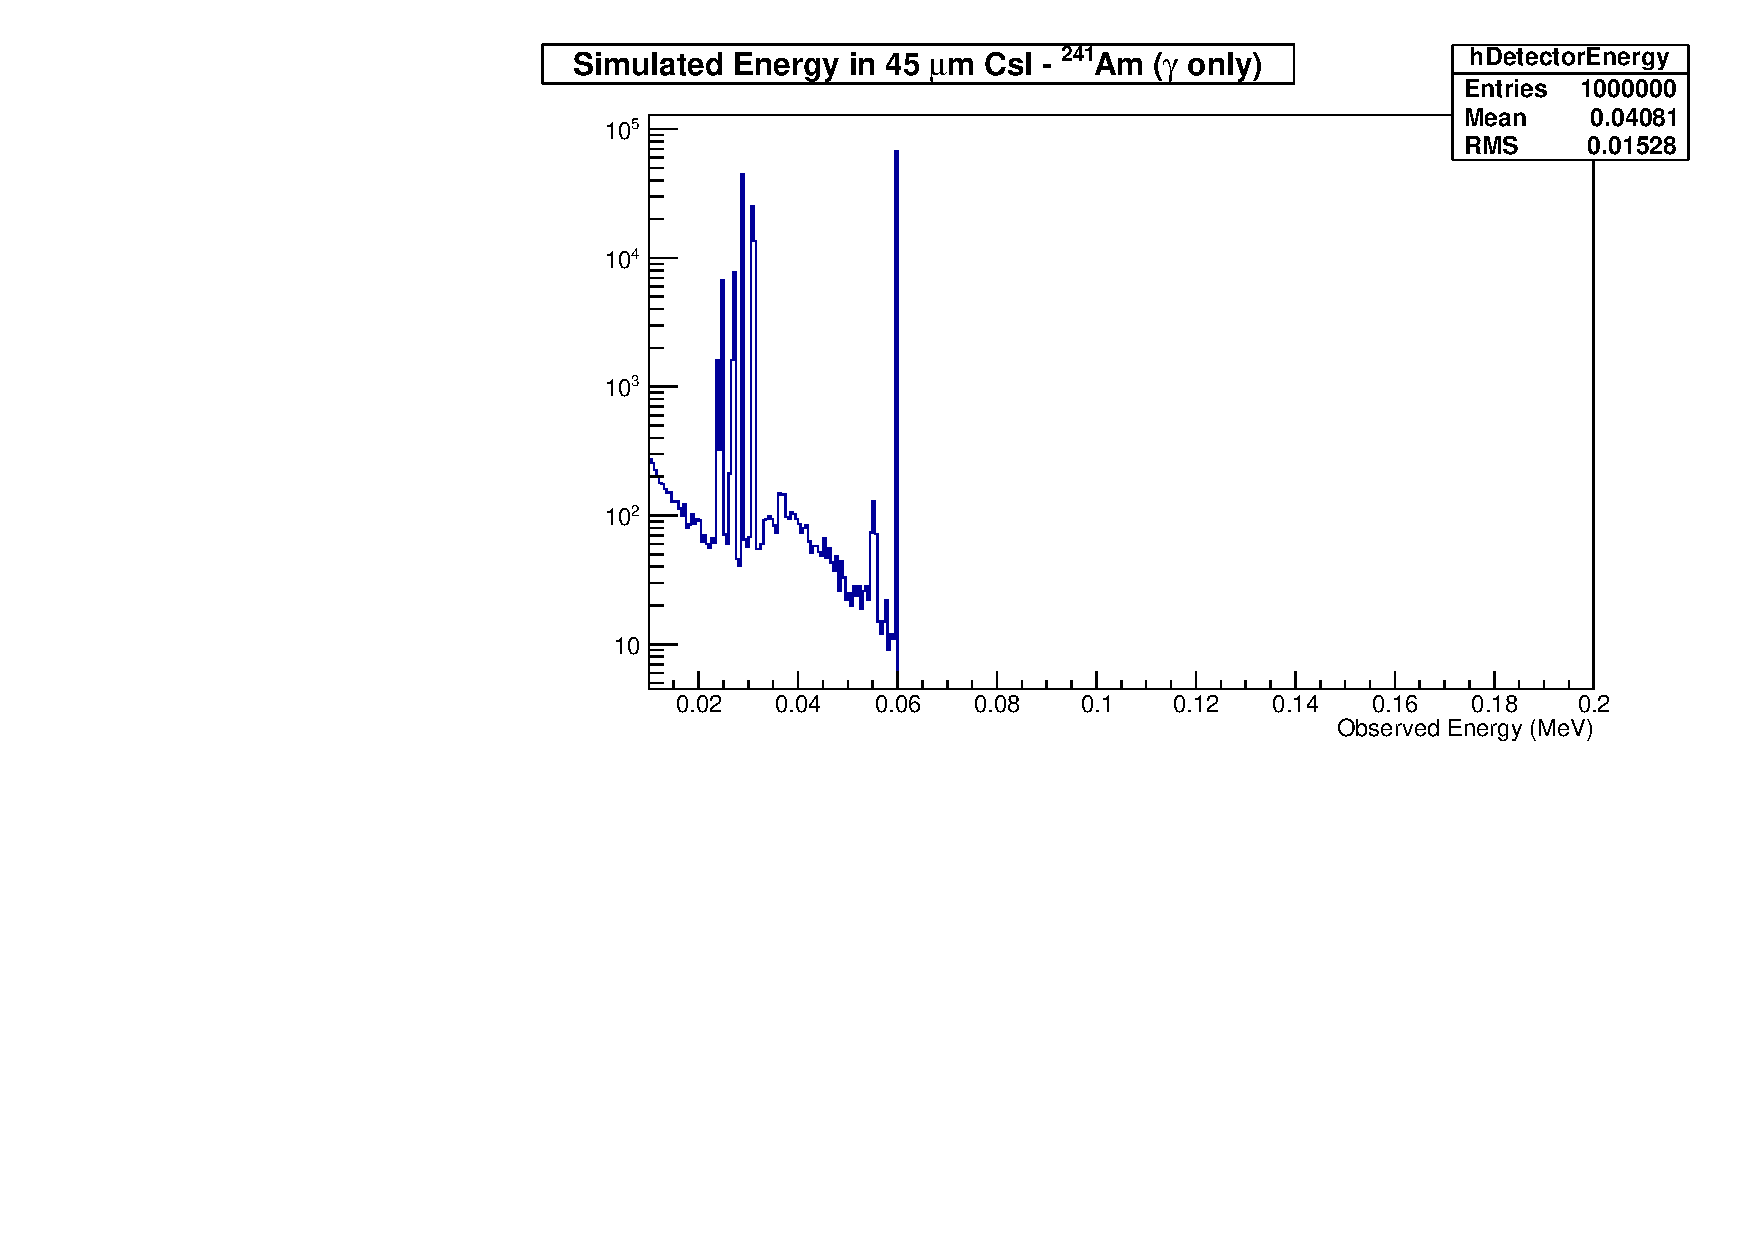
\includegraphics[width=0.45\textwidth]{sim_plots/Am241-45micron.pdf} }}
      
      \subfigure{{
	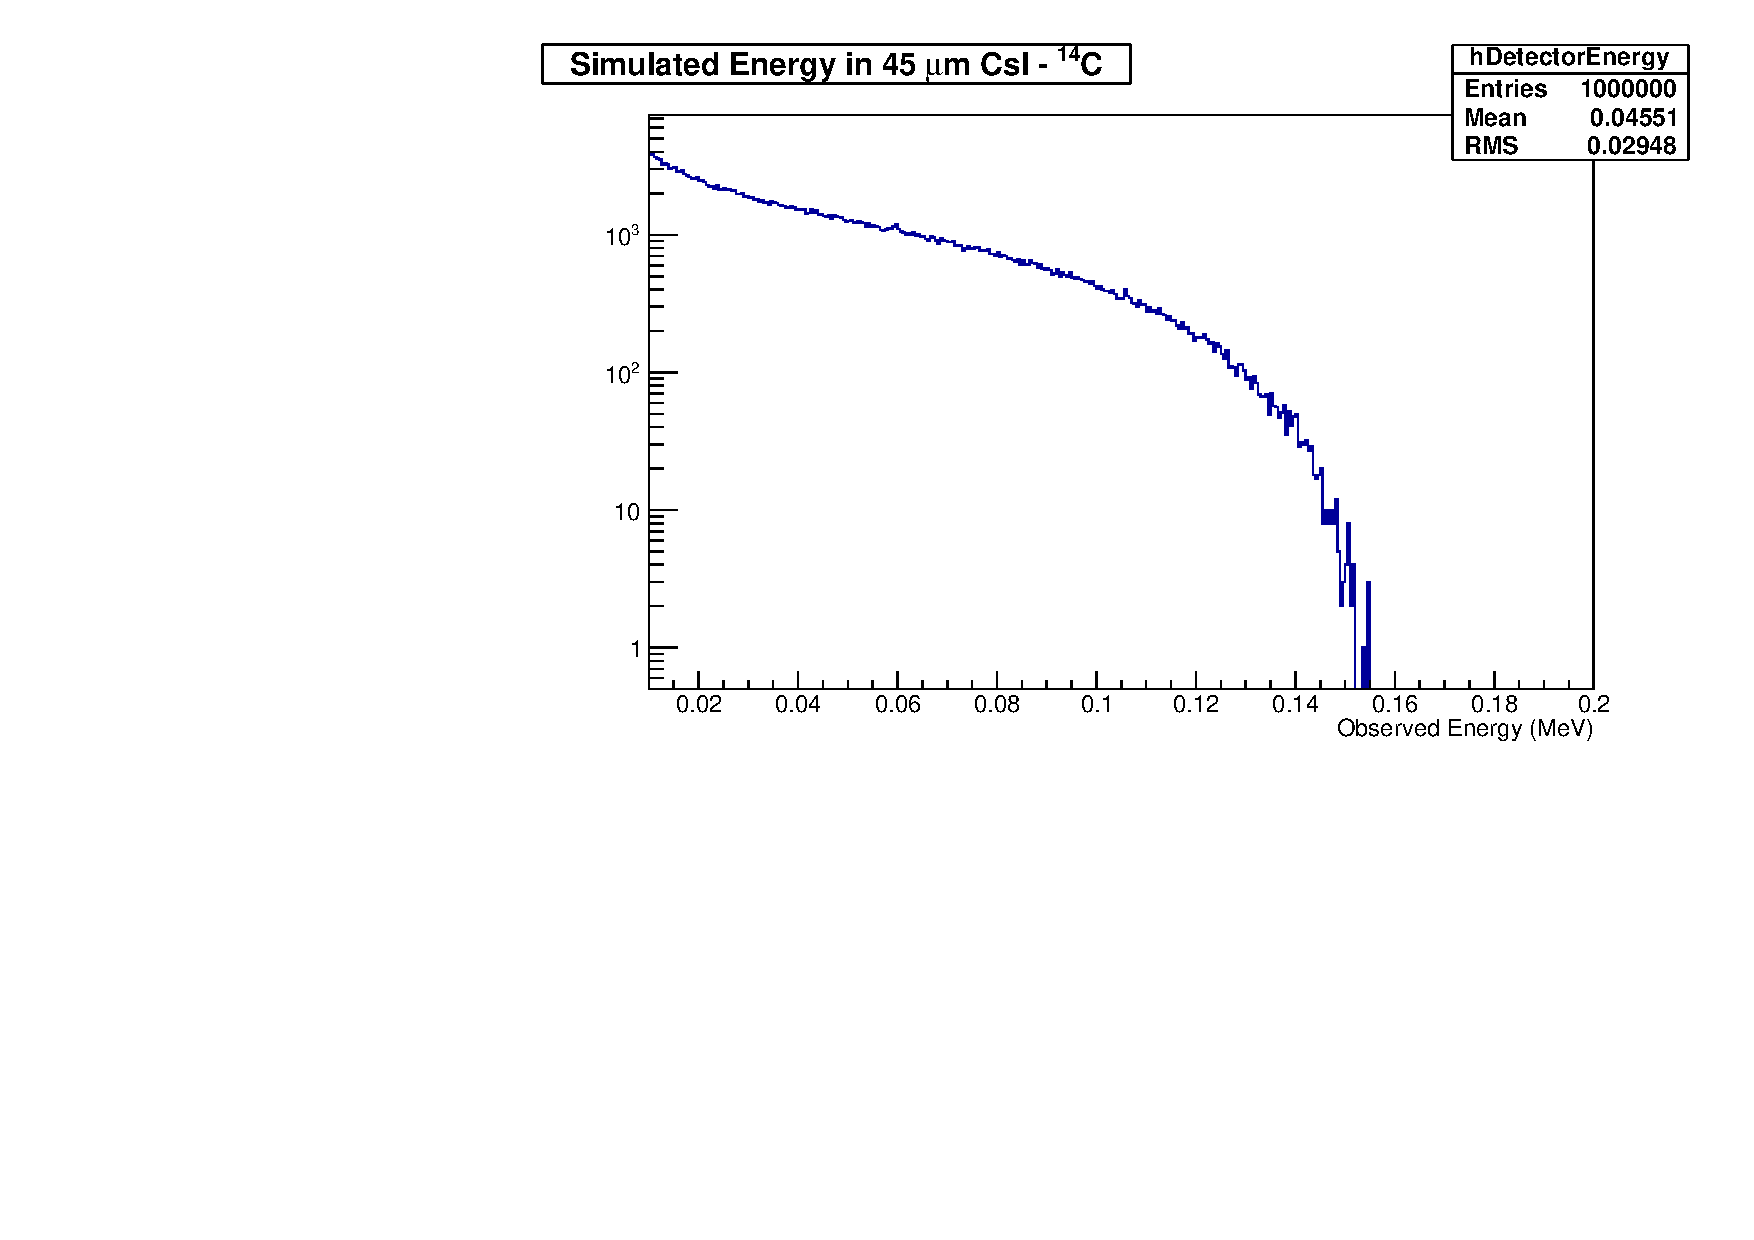
\includegraphics[width=0.45\textwidth]{sim_plots/C14-45micron.pdf}
	      }}
       \subfigure{{
        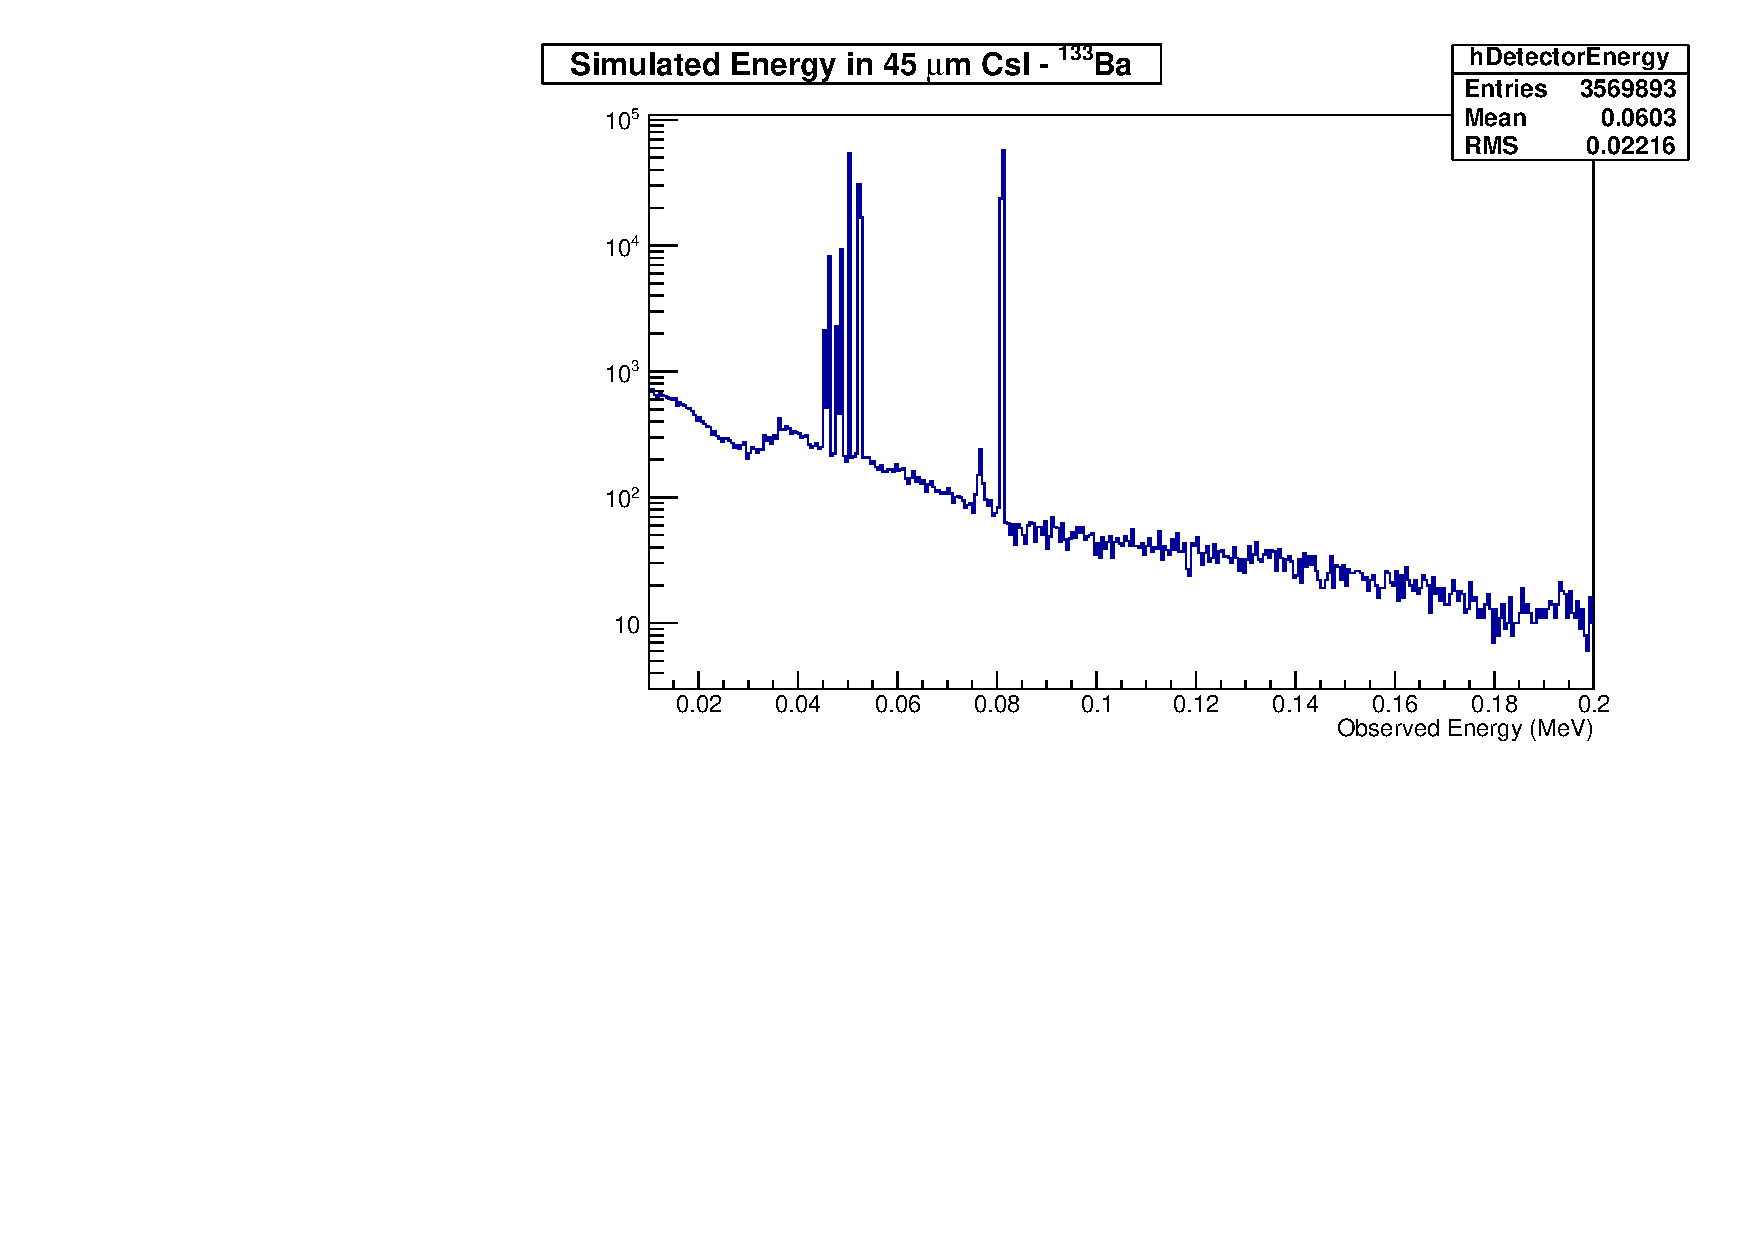
\includegraphics[width=0.45\textwidth]{sim_plots/Ba133-45micron.pdf}
       	      }}    
	\subfigure{{
	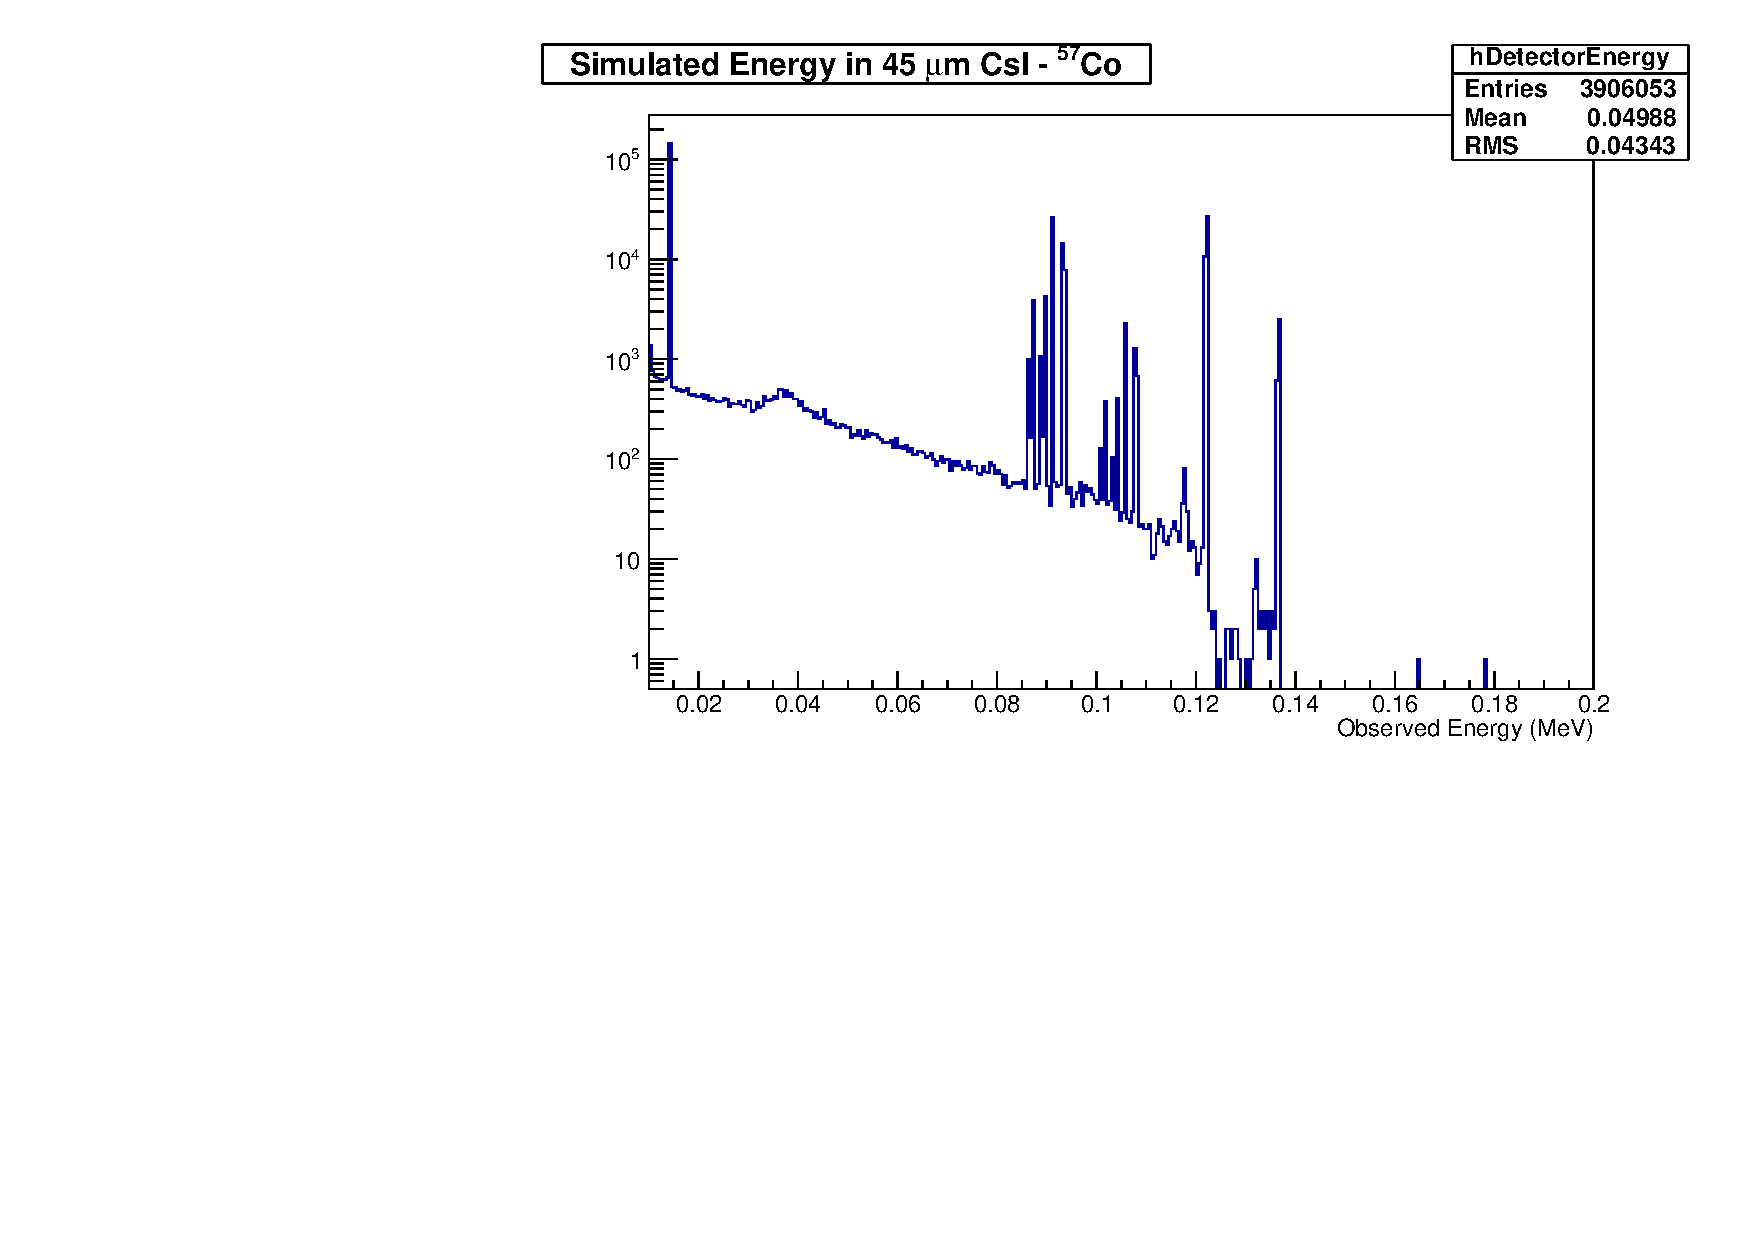
\includegraphics[width=0.45\textwidth]{sim_plots/Co57-45micron.pdf}
	}}	      
	\subfigure{{ 
	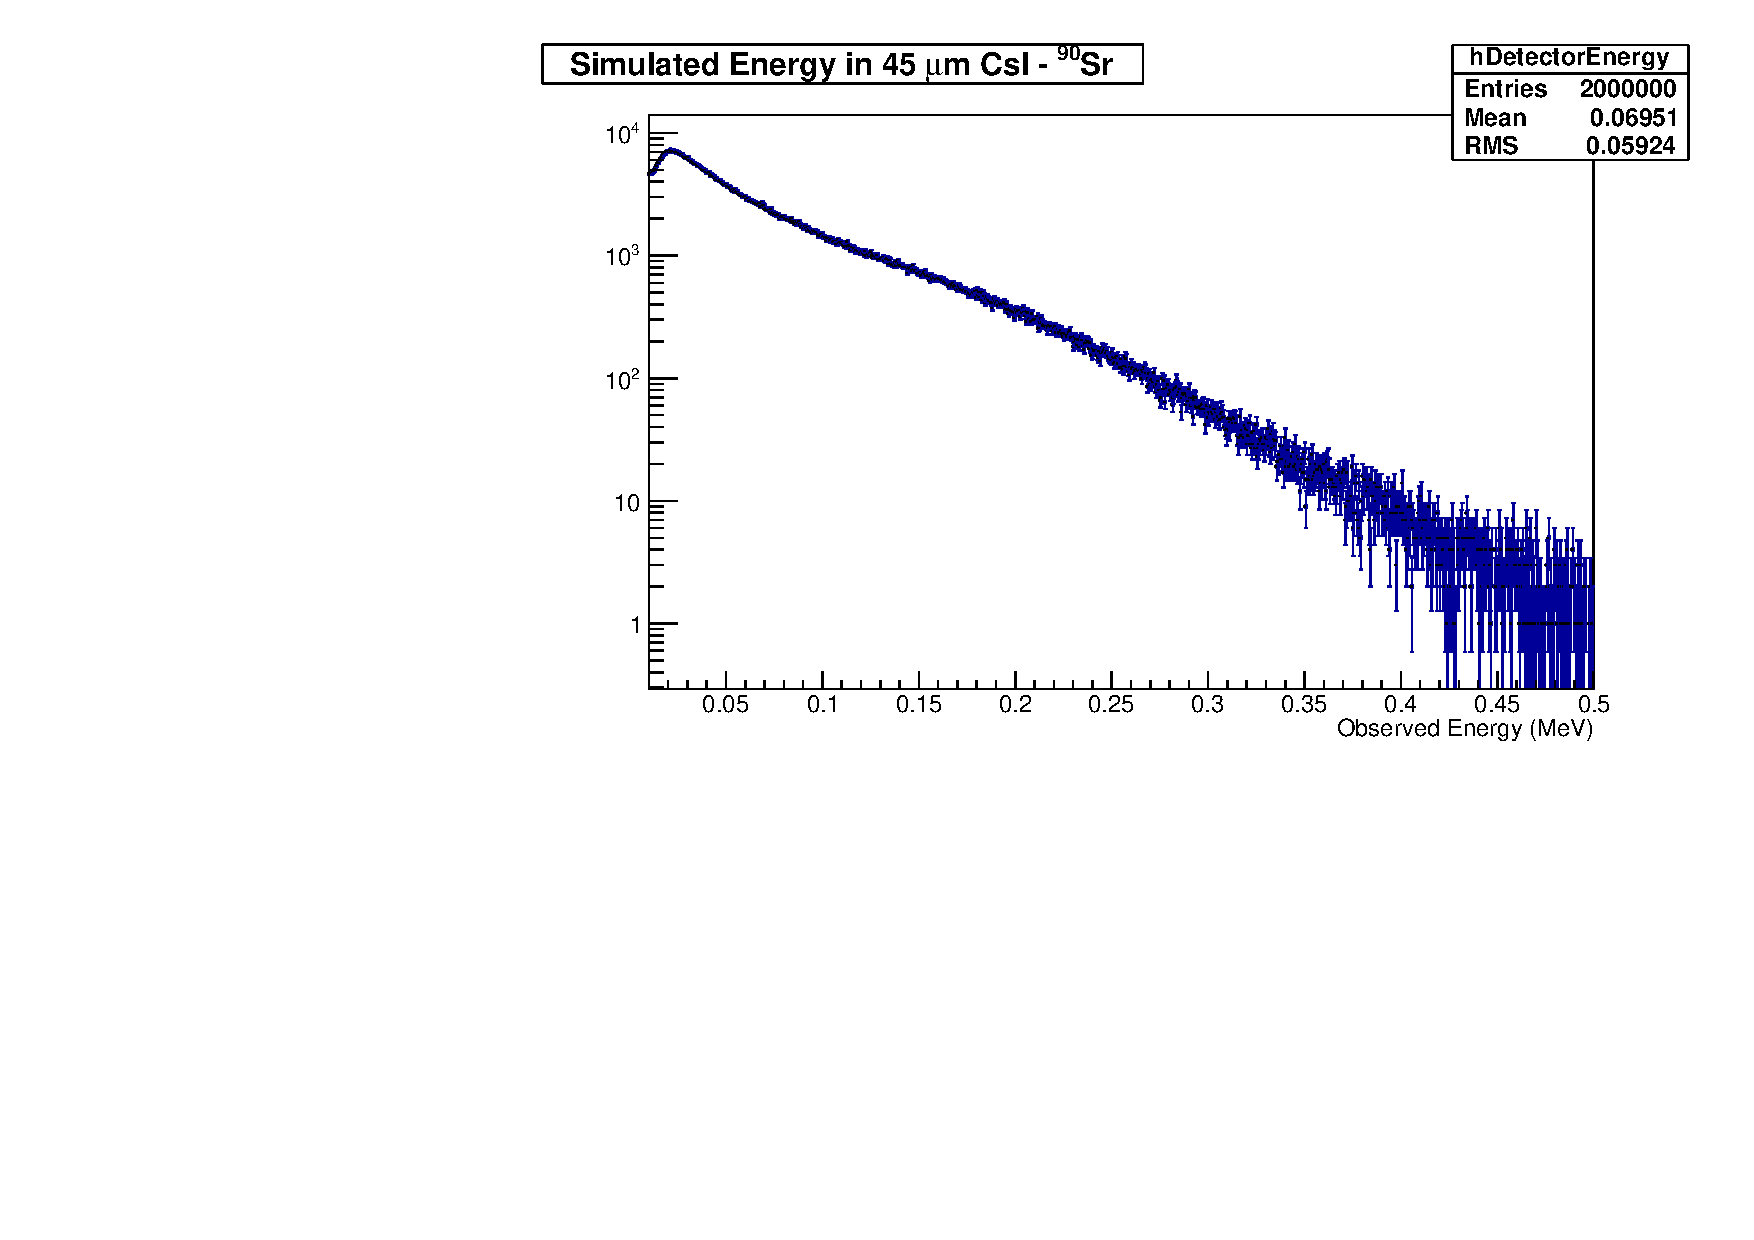
\includegraphics[width=0.45\textwidth]{sim_plots/Sr90-45micron.pdf}	
	}}
	\caption{Simulated energy spectra in 45 $\mu$m thick CsI for a variety of calibration sources available at LANL
           }
       \label{pic:simulated_spectra}
   \end{center}    
 \end{figure} 


\section{Optical Model}
\emph{Information to be added. Add discussion of flux collected as a function of N.A.}


\section{Results}
The studies conducted with SLIMER thus far have focused on the background present in the system, attempts to determine the energy scale of the system, and finally attempts to observe \nuc{14}{C} decays as well as other low energy events such as \nuc{241}{Am} gamma rays. 

\subsection{Background Study}
The sources of background were studied. The possible sources of background in this experiment include:
\begin{itemize}
\item EMCCD noise (electronic noise, ``dark current'',  clock induced charge, etc)
\item Stray light caused by light leaks  
\item Actual scintillation events from background radiation
\end{itemize}
\subsubsection{EMCCD Noise}
EMCCD noise was studied by collecting data with the EMCCD camera shutter closed. It should be noted that the camera shutter can be rotated closed 	\emph{without} activating the camera's Quick Calibration feature by performing this step with the Nikon Elements software running and communicating with the camera.

We study the histogram of pixel counts, plotted for every pixel in a image, over a large number of images.
The mean value and tail indicate the level of noise present in the EMCCD system. We also study the time dependence of the noise by plotting the mode, median and mean of the pixel counts per image
as a function of time. REPEAT THE STUDY, AND ADD THE HISTOGRAM OF PIXEL COUNTS

We also examine how this noise contributes to the actual background by creating ``false'' events where the noise mimics an actual scintillation event. We run our image analysis code on the above data, attempting to reconstruct scintillation-like events. DO THIS STUDY, AND SHOW THE ENERGY SPECTRUM, NORMALIZED TO TIME, OF THE RESULTING RECONSTRUCTED EVENTS.

\subsubsection{Stray Photons}
We study stray light caused by light leaks by opening the EMCCD camera shutter, and collecting events \emph{without} the CsI in place. Again, we study the histogram of pixel counts, for every pixel in a image, over a large number of images. The resulting distribution of pixel counts when compared to the same plotted for data collected with the shutter closed reveals the effect due to stray light. We study the time dependence of the light by plotting the mode, median and mean of the pixel counts per image
as a function of time. REPEAT THE STUDY, AND ADD THE PLOT
We also examine how this stray light contributes to the actual background by creating ``false'' events where the light mimics an actual scintillation event.   We run our image analysis code on the above data, attempting to reconstruct scintillation-like events. DO THIS. 

\emph{Consider if using the shutter integrated with the filter wheel assembly will tell us anything. If the shutter is located above the filter wheel, just below the objective lens, then collecting data with this shutter closed and comparing it with the shutter open would ID light leaks coming from inside the microscope or outside.}

\subsubsection{Background Radiation}
Finally, we study the effect of background radiation by adding the CsI slide to the system. Again, we study the histogram of pixel counts, for every pixel in a image, over a large number of images.
DO THIS, WITH ALL THREE SCINTILLATOR SLIDES. 

\subsubsection{Summary of Background Studies}
ESTIMATE THE MAIN BACKGROUND CONTRIBUTION HERE. THE ID OF THE MAIN SOURCE OF BACKGROUND WILL REVEAL IF WE CAN LOWER THE BACKGROUND.

\subsection{14C spectra and efficiency}%%%%%%%%%%%%%%%%%%%%%%%%%%%%%%%%%%%%%%%%%%

In order to understand the signature of \nuc{14}{C} scintillation in the SLIMER apparatus, we collect data with the two thin window \nuc{14}{C} sources in order to achieve high rates relative to background. 

\subsubsection{High rate \nuc{14}{C} source in direct contact with CsI} 
Data were collected with the high intensity source resting directly atop of the CsI in order to produce the maximum rate of \nuc{14}{C} beta interactions in the CsI. The rate was further optimized by manually scanning the telescope  across the CsI until the rate of interactions seen with the DAQ software subjectively appeared to be the highest. The magnification of this run was 20x with an EM gain of 200. 
Data were collected with the source in place, and then an background exposure was done with the source removed. The resulting spectrum is shown in Figure \ref{pic:high_rate_c4_no_collimator_spectrum}.

\begin{figure}[h!p] 
  \begin{center}     
   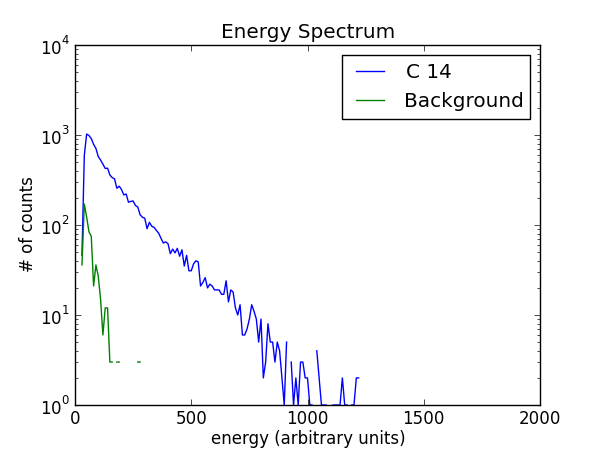
\includegraphics[]{eriks_plots/cluster_smooth_plot_8_13_2013.png}
	\caption{The observed energy spectrum in arbitrary units with the high rate \nuc{14}{C} calibration source, after a three hour run. The energy estimate is made by integrating the pixel counts within a cluster. The background is also shown for comparison purposes, and was taken during an one hour run and scaled up by a factor of three for comparison purposes.. From this plot it is clear that there is a excess of events, indicating observation of \nuc{14}{C} beta decays in SLIMER.  
           }
       \label{pic:high_rate_c4_no_collimator_spectrum}
   \end{center}    
 \end{figure} 


\subsubsection{High rate \nuc{14}{C} source in 1.0 mm collimator} 
Data were collected with the high intensity source resting in the 1mm diameter copper collimator, which in turn was placed within the source, scintillator, collimator (SSC) assembly
The rate was NOT optimized by scanning,
instead a random point aligned with the collimator hole was selected. The magnification of this run was 20x with an EM gain of 200. 
Data were collected with the source in place, and then an background exposure was done with the source and SSC removed, and with the CsI placed directly on the stage.
The resulting spectrum is shown in Figure \ref{pic:high_rate_c4_1mm_collimator_spectrum}.
\begin{figure}[h!p] 
  \begin{center}  
    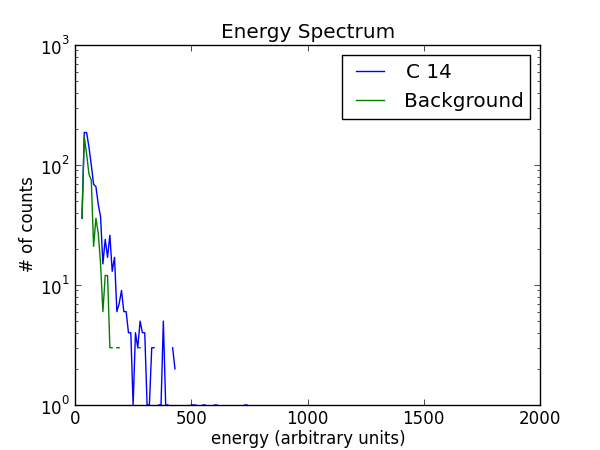
\includegraphics[]{eriks_plots/cluster_smooth_plot_coll_8_13_2013.png}
     	\caption{The observed energy spectrum in arbitrary units with the high rate \nuc{14}{C} calibration source paired with the 1mm collimator,. The energy estimate is made by integrating the pixel counts within a cluster. The background is also shown for comparison purposes.            }
       \label{pic:high_rate_c4_1mm_collimator_spectrum}
   \end{center}    
 \end{figure} 


\subsubsection{High rate \nuc{14}{C} source in 0.250 mm collimator} 
%Data were collected with the high intensity source resting in the 0.250 mm diameter copper collimator, which in turn was placed within the CsI/collimator assembly. The rate was NOT optimized by scanning,
%instead a random point aligned with the collimator hole was selected. The magnification of this run was XXXX with an EM gain of XXXX. 
%Data were collected with the source in place, and then an background exposure was done with the source removed, but the collimator/CsI assembly still in place. 
\begin{comment}
\begin{figure}[h] 
  \begin{center}      
     	\caption{The observed energy spectrum in arbitrary units with the high rate \nuc{14}{C} calibration source paired with the 0.25 mm collimator, normalized to exposure time. The energy estimate is made by integrating the pixel counts within a cluster. The background is also shown for comparison purposes.            }
       \label{pic:high_rate_c4_point25mm_collimator_spectrum}
   \end{center}    
 \end{figure} 
 \end{comment}

 
 
 
 \subsubsection{Low rate \nuc{14}{C} source in direct contact with CsI} 
%Data were collected with the low intensity source resting directly atop of the CsI in order to produce a more realistic rate of \nuc{14}{C} beta interactions in the CsI. The rate was optimized by manually scanning %the telescope  across the CsI until the rate of interactions seen with the DAQ software subjectively appeared to be the highest. The magnification of this run was XXXX with an EM gain of XXXX. 
%Data were collected with the source in place, and then an background exposure was done with the source removed. 

\begin{comment}
\begin{figure}[h] 
  \begin{center}      
     %\mbox{
     \subfigure{\scalebox{0.25}{
	%\includegraphics{plots/egamp_plot3.eps}
      }}
      \subfigure{\scalebox{0.25}{
	%\includegraphics{plots/tau_plot2.eps}
      }}
      %}
	\caption{The observed energy spectrum in arbitrary units with the low rate \nuc{14}{C} calibration source, normalized to exposure time. The energy estimate is made by integrating the pixel counts within a cluster. The background is also shown for comparison purposes. From this plot it is clear that there is a excess of events, indicating observation of \nuc{14}{C} beta decays in SLIMER.  
           }
       \label{pic:high_rate_c4_no_collimator_spectrum}
   \end{center}    
 \end{figure} 
\end{comment}
 
\subsubsection{Low rate \nuc{14}{C} source in 0.250 mm collimator, edge of collimator imaged} 
%Data were collected with the low intensity source resting in the 0.250 mm diameter copper collimator, which in turn was placed within the CsI/collimator assembly. The rate was NOT optimized by scanning,
%instead the edge of collimator was imaged. Not only does this permit an estimate of the spatial resolution at low energies, but also provides a final check against the signal: the \nuc{14}{C} candidates should %reconstruct in the open area of the collimator. 

%The magnification of this run was XXXX with an EM gain of XXXX. 
%Data were collected with the source in place, and then an background exposure was done with the source removed, but the collimator/CsI assembly still in place. 

\subsubsection{Discussion of \nuc{14}{C} Results}
It is clear that we have a number of different runs in which the event rate is increased and the energy spectrum is significantly broadened when the high rate \nuc{14}{C} source is present, compared to background runs without the source present. 
These two observables strongly indicate that SLIMER is indeed very capable of observing \nuc{14}{C} decays, in the very least with activities of 1 $\mu$Ci and greater.  

However the current round of studies indicates a very strong variation in both event rate and energy spectrum for \nuc{14}{C} decays. The origin of these variations is not presently understood.
As the goal of this project is to reliably determine the \nuc{14}{C} activity in arbitrary samples, these variations need to be understood and addressed.  
Once we have can produce reproducible estimates of the \nuc{14}{C} AND background spectra, we can project our sensitivity as a function of \nuc{14}{C} activity, \nuc{14}{C} density and exposure.
 
\subsection{\nuc{241}{Am} ($\gamma$ only) spectra and efficiency}
%Data were collected with the sealed \nuc{241}{Am} $\gamma$ source. Here we exploit the 59.6 keV $\gamma$ line present in the \nuc{241}{Am} decay, assume no other lines are present, and note that this
%source will not permit $\alpha$ particles to escape. 

%The magnification of this run was XXXX with an EM gain of XXXX. 
%Data were collected with the source in place, and then an background exposure was done with the source removed. 

\begin{comment}
\begin{figure}[h] 
  \begin{center}      
     %\mbox{
     \subfigure{\scalebox{0.25}{
	%\includegraphics{plots/egamp_plot3.eps}
      }}
      \subfigure{\scalebox{0.25}{
	%\includegraphics{plots/tau_plot2.eps}
      }}
      %}
	\caption{The observed energy spectrum in arbitrary units with the \nuc{241}{Am} calibration source, normalized to exposure time. 
           }
       \label{pic:am_241_gamma_spectrum}
   \end{center}    
 \end{figure} 
 \end{comment}

\subsection{\nuc{90}{Sr} spectra and efficiency}
%Data were collected with the large \nuc{90}{Sr} beta source. Both the \nuc{90}{Sr} and daughter \nuc{90}{Y} decays are expected to deposit more energy in the CsI than either the \nuc{14}{C} or \nuc{241}{Am} %sources. 

%This source is quite large, so the alignment procedure is amended: first the source is placed atop the CsI, and then the overhead light in the microscope is used to center the source. 
%The magnification of this run was XXXX with an EM gain of XXXX. 
%Data were collected with the source in place, and then an background exposure was done with the source removed. 
\begin{comment}
\begin{figure}[h] 
  \begin{center}      
     %\mbox{
     \subfigure{\scalebox{0.25}{
	%\includegraphics{plots/egamp_plot3.eps}
      }}
      \subfigure{\scalebox{0.25}{
	%\includegraphics{plots/tau_plot2.eps}
      }}
      %}
	\caption{The observed energy spectrum in arbitrary units with the \nuc{90}{Sr} calibration source, normalized to exposure time. 
           }
       \label{pic:sr_90_spectrum}
   \end{center}    
 \end{figure} 
\end{comment}

\subsection{\nuc{207}{Bi} spectra and efficiency}
%Do we have data in the can to show this? 
 
 
\subsection{\nuc{241}{Am} $\alpha$ source } 
%Data were collected with the thin window \nuc{241}{Am} $\alpha$ source. Here, we would expect near full energy deposition into the CsI. 

%The magnification of this run was XXXX with an EM gain of XXXX. 
%Data were collected with the source in place, and then an background exposure was done with the source removed. 


WANT TO SHOW ALPHA SENSITIVITY AS A FUNCTION OF EXPOSURE TIME, BACKGROUND RATE AND SOURCE STRENGTH.

\section{Study and Comment Regarding Earlier Work on SLIMER}
For the first time, \nuc{14}{C} decay candidates have been observed with SLIMER. The signal, under optimum conditions, is quite clear. It is interesting to ask why the signal was not previously observed.
The main difference in this study, compared to previous work is the operating temperature of the EMCCD (we ran at -80C and below), magnification (we ran at 20x versus 4x), set EM gain (we ran at 200x versus 1000x) and BERT setting (not used here, versus using a threshold of 1.2-1.4 previously).

A quick visual study was conducted with the high intensity \nuc{14}{C} source in SLIMER. The Live View mode of Elements was utilized to visually inspect the data. \nuc{14}{C} candidates could be readily seen at 20x magnification, even without the camera fully cooled to -80C or below. Typical cluster sizes were observed to be 5x5 pixels. Upon reducing the magnification to 10x, the \nuc{14}{C} candidates could still be seen. However, at 4x magnification no \nuc{14}{C} candidates were apparent.  BERT was not used at this time. 

This quick study invites two hypotheses regarding the apparent success of the latest work on SLIMER. One is that the reduced magnification also reduced the light collection from scintillation events and essentially shifted the \nuc{14}{C} into the background. Since the flux collected by an optical system goes as the square of the numerical aperture, the 20x magnification setting can be expected to collect nearly 15 times more light than the 4x setting. Second, BERT could be expected to suppress many of the \nuc{14}{C} candidates at low magnification. The 5x5 pixel clusters observed at 20x magnification would instead map to a single pixel at 4x magnification.  However, large single pixels are just the type of event that BERT, a median filter, is designed to suppress. 

Ignoring other factors which may also play a role, it appears that low magnifications and the use of BERT would be sufficient to suppress or eliminate \nuc{14}{C} candidates.    


      
 
  
\section{Observed Problems}
Over the past two months, we may have discovered a number of complications in the running of the SLIMER apparatus. These complications should be confirmed and mitigated in the future.

\subsection{Light Leaks}
A shift in the mode of the pixel count histogram was observed when the camera shutter is opened. This indicates a light leak of some type. 

\subsection{Communication Problems}
The Nikon Elements DAQ software is able to control the filter wheel position. Upon startup, the filter wheel may rotate to a random position. This is a concern as the transmission of 
light through the two existing filter cubes as well as empty slots can be expected to be quite different and would thus impact the observed energy scale.
This can be checked by using the Nikon Element controls, and mitigated by adding this check to the startup procedure. However, this possibility should be factored in
when dealing with older data sets. 


\subsection{Camera Driver Issues}
There appears to be an issue with the Camera Driver, as it sometimes crashes and kills a run. The error message is error ``-9''.

\subsection{Windows Power Management Settings}
STOW may be setting the power management options in such a way that renders overnight runs difficult. It is unclear if this problem is due to the monitor shutting off, or the computer being put to sleep.


\subsection{Strong temperature dependence}
A strong EMCCD temperature dependence is suspected, with lower temperatures results in a higher \nuc{14}{C} observation rates. This needs to be checked. 

\subsection{Focusing Problems}
We have seen signs that the focus at the 20x setting changes when the source is placed/removed. Not touching the scintillator slide seems to help, but this may be a weight issue.
We confirmed that there is NOT a time-dependent drift in focus. This is mitigated when using the SSC, but will be an issue if bare sample or sources are placed atop the CsI. 

\subsection{Varying Background Level}
We have found evidence for a difference in the variance on the background level (the raw pixel counts) between two background runs taken during different days. 
The shift in variance is from 7 to 10 counts/pixel. We have also seen evidence of a shift in the mean pixel counts on an image by image basis. This agrees with
the observation of a shifting pixel count histogram within the Nikon Elements DAQ software.

\subsection{Varying \nuc{14}{C} rate}
Different \nuc{14}{C} event rates have been observed, as well as different end points in the energy spectra, during different runs. 


\subsection{Optimum Magnification}
We have consistently been able to produce good observations at 20x magnification, with few background events satisfying our analysis criteria. However, to check if this magnification was optimum, we also ran at 10x magnification, with all other DAQ settings the same. For these data, a shift in the energy spectra was observed. While this is expected due to the different numerical apertures of the objective lenses and hence different amounts of light collection, the shift observed may have been larger than expected. 

\subsection{Decrease in rate due to use of collimator}
Even when the field of view is not occluded, we observe a substantial decrease in event rate when the \nuc{14}{C} sources are used with a collimator. This is likely due to some combination of 
effective sample area on the source, solid angle, as well as scattering effects. This needs to be understood, or at least well measured so that we can better estimate the conversion between event rate and source activity.

\subsection{Background cluster sizes}
We observed that the clustering algorithm would typically find clusters of two different sizes in the background data. One is likely CIC events. Plotting the energy of the cluster versus the size may better separate these two classes of events. 

\section{To Do List}
In order of priority:
\begin{enumerate}
\item Re-analyze original noise data.
\item Repeat EMCCD noise study, and add in time dependence
\item Repeat light leak study, add in time dependence and perhaps use filter wheel shutter
\item Repeat background study with the three scintillators.
\item QuantView study: QuantView is a feature present in the EMCCD camera in which the signal is output in units of photoelectrons detected per pixel. This feature may eliminate the need for pixel by pixel background subtraction, and also factors in different camera settings. Using this feature may then permit more consistent data taking and may make studies in which camera parameters are scanned easier to interpret.  If the output is straightforward to interpret, this should be used from this point forward. A data run with the high intensity \nuc{14}{C} source should be run in this mode, as well as a background run.
\item Reproducibility studies --- CsI spatial uniformity:
	\begin{itemize}
		\item \nuc{14}{C} data collected with 250 $\mu$m collimator: different runs in different positions within the hole, compare energy scale and rate of samples.
		\item \nuc{14}{C} data collected with 1mm	 collimator: different runs in different positions within the hole, compare energy scale and rate of samples.
		\item \nuc{14}{C} data collected without collimator, but source raised above CsI: different runs in different positions, compare energy scale and rate of samples. 
	\end{itemize}
The above data seek to probe the CsI light yield as a function of position.	 
\item Code to extract camera temperature from frame
\item Code to extract exposure time from frame.
\item Reproducibility studies --- Time Stability: \item \nuc{14}{C} data collected with 1mm	 collimator over 8 hours. Study energy spectrum and rate over this time period. If variation is present,
check for correlation with camera temperature (extracted using new code).
\item Reproducibility studies --- Day to Day Stability: \item \nuc{14}{C} data collected with 1mm collimator over multiple days, with camera and equipment power cycling in between.	 
Study energy spectrum and rate for each sample and compare.
\item High/ Low Intensity \nuc{14}{C} spectra.....then scale to expected activity level from samples. 
\item Alpha energy + resolution.... assume spread due to photon statistics, estimate light yield. Compare to simulation.
\item Estimate Run time required for phylochip study
\item Collect more data, in particular \nuc{57}{Co}, \nuc{207}{Bi}, \nuc{137}{Cs} and \nuc{241}{Am} alphas
\item BERT study, as a function of magnification.
\item Performance/rate as a function of magnification.
\item Fluorescence testing , require proper dyes.
\item Spatial resolution using collimator
\item Code to look at mode and spread of pixel counts per image, as a function of time.
\item Determine low energy threshold of SLIMER. 
\item Measure C14 event rate and energy spectrum (as well as background) as a function of magnification, EM gain, conversion gain, and temperate. 
\item Do ESR foil study, and estimate the amount of light lost through the top of the CsI. 
\item Produce a good sample of images of different classes of events (background, C14, Am241, Sr90, Cs137 and alphas) with the pixels counted as the event highlighted. Both smoothed and unsmoothed data should be displayed, and this should be done at different magnifications. 
\item Understand if we want to keep overlapped frames
\item Study EMCCD clear mode
\item Study gain as a function of temperature, and refer to Mary's email thread with Photometrics. 
\item Study the effect of clearing when running on "overlap" mode.   
\item CsI light yield temperature dependence AT LOW ENERGIES.
\end{enumerate} 
 
 

%\subsection{}



\end{document}  